\documentclass[10pt]{report}
%%%%%%%%%%%%%%%%%%%%%%%%%%%%%%%%%%%%%%%%%%%%%%%%%%%%%%%%%%%%%%%%%%%%%%%%%%%%%%%%
% LaTeX Includes
%%%%%%%%%%%%%%%%%%%%%%%%%%%%%%%%%%%%%%%%%%%%%%%%%%%%%%%%%%%%%%%%%%%%%%%%%%%%%%%%
\usepackage{amsmath}    % Math formatting
\usepackage{amsthm}     % Math Theorems
\usepackage{amsfonts}   % Math formatting
\usepackage{amssymb}    % Math formatting
\usepackage{setspace}   % Allow double spacing
\usepackage{graphicx}   % Include images
\usepackage{times}      % Use Times New Roman font
\usepackage[margin=1in]{geometry}
\usepackage{pdfpages}   % Include pdfs
\usepackage{tikz}       % Create Pictures
\usepackage{pgfplots}   % Create Pictures
\usepackage{caption}    % Figure captioning
\usepackage{subcaption} % Figure captioning
\usepackage{media9}     % include animated .gifs
\usepackage{attachfile} % AttachFiles
\usepackage{tocloft}    % List of Equations
\usepackage{listings}   % Fancy Code display
\usepackage{color}      % Fancy Colors
\usepackage{fancyhdr}   % Fancy Header
\usepackage{microtype}  % Fancy spacing
\usepackage{hyperref}   % Reference
\hypersetup{hidelinks}
\RequirePackage[l2tabu, orthodox]{nag} % Nag about bad syntax
\renewcommand*\thesection{\arabic{section}} % Renew Section numbers for report class
%%%%%%%%%%%%%%%%%%%%%%%%%%%%%%%%%%%%%%%%%%%%%%%%%%%%%%%%%%%%%%%%%%%%%%%%%%%%%%%%
% Custom commands
%%%%%%%%%%%%%%%%%%%%%%%%%%%%%%%%%%%%%%%%%%%%%%%%%%%%%%%%%%%%%%%%%%%%%%%%%%%%%%%%
\newcommand{\nvec}[1]{\left\langle #1 \right\rangle}        % Easy to use vector
\newcommand{\abs}[1]{\left\lvert #1 \right\rvert}           % Easy to use abs
\newcommand{\pren}[1]{\left( #1 \right)}                    % Big parens
%%%%%%%%%%%%%%%%%%%%%%%%%%%%%%%%%%%%%%%%%%%%%%%%%%%%%%%%%%%%%%%%%%%%%%%%%%%%%%%%
% Beginning of document items - headers, title, toc, etc...
%%%%%%%%%%%%%%%%%%%%%%%%%%%%%%%%%%%%%%%%%%%%%%%%%%%%%%%%%%%%%%%%%%%%%%%%%%%%%%%%
\begin{document}
\pagestyle{fancy}
\fancyhead[LE,LO]{APPM 2360 - Differential Equations}   % Adds header to left
\fancyhead[RE,RO]{Project Two - Matrices}               % Adds header to right

\title{Image Manipulation Using Matrix Techniques}
\author{
\begin{tabular}{l | l | l | l | l}
    Names & Student ID & Professor & TA & Recitation\\
    \hline
    Will Farmer & 101446930 & Mimi Dai & Amrik Sen & 608\\
    \hline
    Jeffrey Milhorn & 100556107 & Kevin Manley & Ed Yasutake & 605\\
    \hline
    Patrick Harrington &100411000 & Mimi Dai & Ash Same & 618\\
\end{tabular}}
\date{Friday, March 22}
\maketitle

\tableofcontents                                                    % These two lines are needed to
\addcontentsline{toc}{section}{Table of Contents}                   % initialize and display TOC
\listoffigures                                                      % These two lines are needed to
\addcontentsline{lof}{section}{List of Figures}                     % initialize and display LOF

\newpage
%%%%%%%%%%%%%%%%%%%%%%%%%%%%%%%%%%%%%%%%%%%%%%%%%%%%%%%%%%%%%%%%%%%%%%%%%%%%%%%%
% Beginning of content
%%%%%%%%%%%%%%%%%%%%%%%%%%%%%%%%%%%%%%%%%%%%%%%%%%%%%%%%%%%%%%%%%%%%%%%%%%%%%%%%

\section*{Introduction}
Since images stored on computers are simply matrices where each element
represents a pixel, matrix methods learned in class can be used to
modify images. The purpose of this project was to apply matrix manipulations
on given image files, shown below as Figure~\ref{fig:p1} and
Figure~\ref{fig:p2}.

\begin{figure}[ht]
  \centering
  \begin{subfigure}{0.6\textwidth}
    \centering
    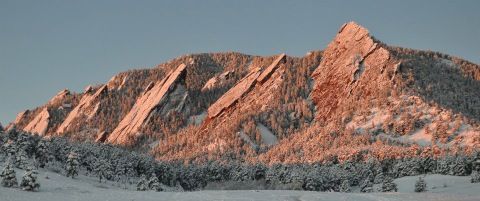
\includegraphics[scale=0.5]{./img/photo1.png}
    \caption{Photo 1}
    \label{fig:p1}
  \end{subfigure}
  \begin{subfigure}{0.3\textwidth}
    \centering
    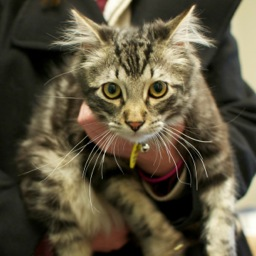
\includegraphics[scale=0.5]{./img/photo2.png}
    \caption{Photo
    2}
    \label{fig:p2}
  \end{subfigure}
  \caption{Provided
  Images}
  \label{fig:init_image}
\end{figure}


\section{Reading Image Files \& Grayscale Conversion}

Colored images have an interesting, although problematic property; they do
not readily lend themselves to matrix             manipulation because in
order to get color images, seperate values are used to represent each primary
color, which are       then mixed together for the final color.  For example,
in Figure~\ref{fig:example}, the block represents very simple a
2$\times$2 pixel image.

\begin{figure}[ht]
  \centering
  
\includegraphics[scale=40]{./img/sqr.png}
  \caption{A simple RGB image}
  \label{fig:example}
\end{figure}

This very simple
image can be
represented as either
a trio of primary
color matrices where
each entry in each
primary        color
matrix coresponds to
the same pixel:

\[  
  \underbrace{
    \begin{bmatrix}
      1&0\\
      0&1\\
    \end{bmatrix}
  }_{\text{Red
  Matrix}}
  ,
  \underbrace{
    \begin{bmatrix}
      0&0\\
      1&1\\
    \end{bmatrix}
  }_{\text{Blue
  Matrix}}
  ,
  \underbrace{
    \begin{bmatrix}
      0&1\\
      0&0\\
    \end{bmatrix}
  }_{\text{Green
  Matrix}}
\]

A
single
matrix
may
be
used,
with
each
entry
being
a
submatrix,
wherein
each
element
in
the
submatrix
corresponds
to
a
primary
color.

\[  
  \begin{bmatrix}
    \begin{bmatrix}1\\0\\0\end{bmatrix}
    &
    \begin{bmatrix}0\\1\\0\end{bmatrix}\\[2em]
    \begin{bmatrix}0\\0\\1\end{bmatrix}
    &
    \begin{bmatrix}1\\0\\1\end{bmatrix}
  \end{bmatrix}
\]

Using
one
of
the
given
images,
the
splitting
of
color
channels
gives
the
following
set
of
images
shown
in
Figure~\ref{3color}.

\begin{figure}[ht]
  \centering
  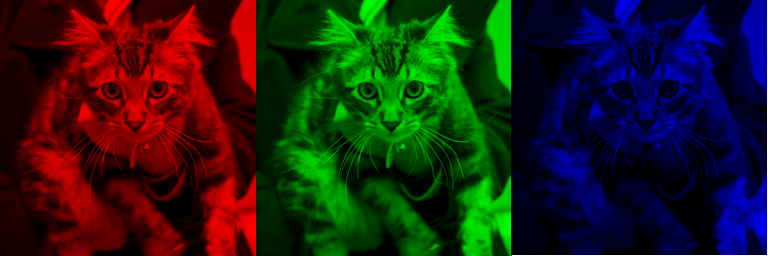
\includegraphics[scale=0.6]{./img/photo2-exploded.png}
  \caption{A
    given
    image
    split
    into
    its
    three
    primary
    color
  channels}
  \label{3color}
\end{figure}

While
it
is
possible
to
manipulate
color
images,
it
would
be
far
simpler
to
manipulate
\emph{grayscale}
images,
where
only
the
final
intensity
is
concerned.
To
do
this,
each
color
is
considered
independently
for
its
intensity
alone
as
shown
in
Figure~\ref{3gray},
where
it
may
be
scaled,
and
then
added
together
to
produce
a
final
black-and-white
image,
which
is
a
matrix
where
each
entry
is
a
single
value.
Note
how
the
third
panel
representing
the
blue
color
channel
is
darker
--
this
implies
that
blue
is
a
less
intense
color
in
the
image.

\begin{figure}[ht]
  \centering
  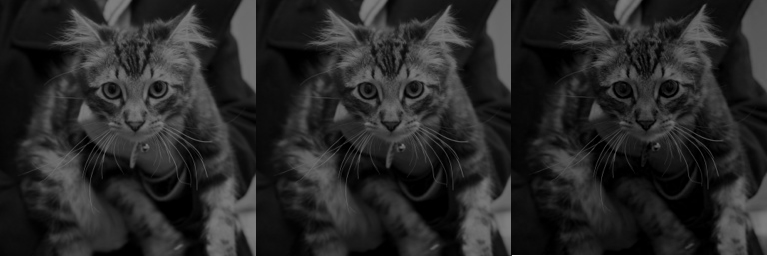
\includegraphics[scale=0.6]{./img/photo2-explodedg.png}
  \caption{A
    given
    image
    split
    into
    its
    three
    primary
    color
    channels,
    but
    only
    intensity
    of
    each
    color
    is
  shown.}
  \label{3gray}
\end{figure}

Since each primary color is freely editable, it is simple to scale the
intensity of each before mixing; in our report, we    used 30\% of the red
channel, 59\% of the green channel and 11\% of the blue channel. The final
outputs for both given       images can be seen in
Figure~\ref{fig:gray_images}. Note how the final output is lighter than any of
the individual color    channels.

\begin{figure}[ht]
  \centering
  \begin{subfigure}{\textwidth}
    \centering
    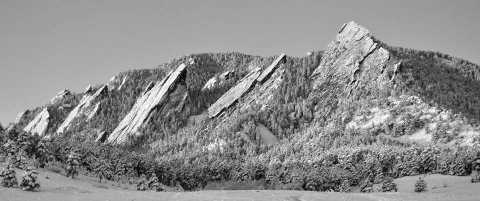
\includegraphics[scale=0.7]{./img/gray1.png}
    \caption{Photo 1 -
    Grayscale}
    \label{fig:p1g}
  \end{subfigure}
  \begin{subfigure}{\textwidth}
    \centering
    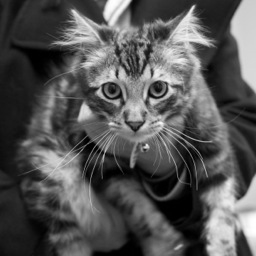
\includegraphics[scale=0.7]{./img/gray2.png}
    \caption{Photo
      2
      -
    Grayscale}
    \label{fig:p2g}
  \end{subfigure}
  \caption{Grayscale
  Images}
  \label{fig:gray_images}
\end{figure}


\section{Horizontal Shifting}

Now that we are working in grayscale, it is far more straightforward to
manipulate aspects of the image, such as its         horizontal position.
Since we are dealing with a normal matrix, transforming the positions of
columns requires only that    we multiply the image matrix by a
transformation identity matrix.

As discussed in the lab instructions, to shift an image horizontally
without
losing information requires the use of a transformation matrix as shown
below.

\[
  \underbrace{
    \begin{bmatrix}
      1&0&0\\
      0&1&0\\
      0&0&1\\
    \end{bmatrix}
  }_{\text{Identity Matrix}}
  \implies
  \underbrace{
    \begin{bmatrix}
      0&1&0\\
      0&0&1\\
      1&0&0\\
    \end{bmatrix}
  }_{\text{Transformation
  Matrix}}
\]

\[ 
  \begin{bmatrix}
    0&0&1\\
    1&0&0\\
    0&1&0\\
  \end{bmatrix}
  \cdot
  \begin{bmatrix}
    a&b&c\\
    d&e&f\\
    g&h&i\\
  \end{bmatrix}
  =
  \underbrace{
    \begin{bmatrix}
      c&a&b\\
      f&d&e\\
      i&g&h\\
    \end{bmatrix}
  }_{\text{the
    horizontally
    shifted
  matrix}}
\]

\begin{figure}[ht]
  \centering
  \begin{subfigure}{\textwidth}
    \centering
    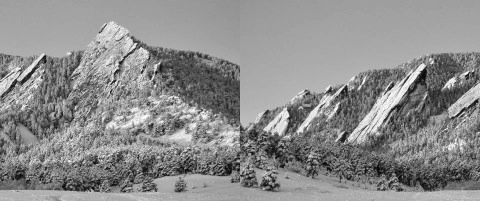
\includegraphics[scale=0.7]{./img/hsg1.png}
    \caption{Photo
      1
      Horizontal
    Shift}
    \label{fig:p1hg}
  \end{subfigure}
  \begin{subfigure}{\textwidth}
    \centering
    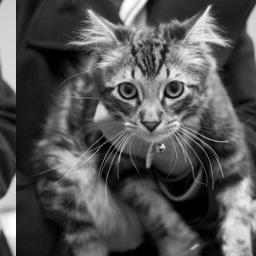
\includegraphics[scale=0.7]{./img/hsg2.png}
    \caption{Photo
      2
      -
      Horizontal
    Shift}
    \label{fig:p2hg}
  \end{subfigure}
  \caption{Horizontally
    Shifted
  Images}
  \label{fig:hs_images}
\end{figure}

\begin{figure}[!ht]
  \centering
  \begin{subfigure}{\textwidth}
    \centering
    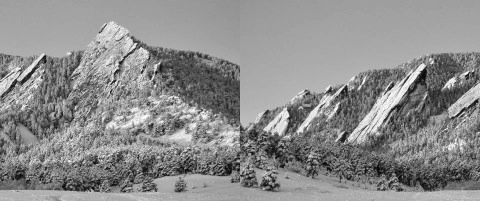
\includegraphics[scale=0.5]{./img/hsg1.png}
    \caption{Photo 1
    Horizontal Shift}
    \label{fig:p1hg}
  \end{subfigure}
  \begin{subfigure}{\textwidth}
    \centering
    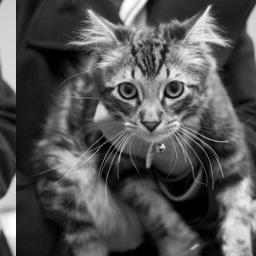
\includegraphics[scale=0.5]{./img/hsg2.png}
    \caption{Photo
      2
      -
      Horizontal
    Shift}
    \label{fig:p2hg}
  \end{subfigure}
  \caption{Horizontally
    Shifted
  Images}
  \label{fig:hs_images}
\end{figure}


\section{Vertical Shifting}

Very similar to the horizontal position change, the vertical position change
merely requires the transformation matrix to be shifted row-wise as opposed
to
column-wise.
\[
  \underbrace{
    \begin{bmatrix}
      1&0&0\\
      0&1&0\\
      0&0&1\\
    \end{bmatrix}
  }_{\text{Identity Matrix}}
  \implies
  \underbrace{
    \begin{bmatrix}
      0&0&1\\
      1&0&0\\
      0&1&0\\
    \end{bmatrix}
  }_{\text{Transformation
  Matrix}}
\]
\[ 
  \begin{bmatrix}
    0&0&1\\
    1&0&0\\
    0&1&0\\
  \end{bmatrix}
  \cdot
  \begin{bmatrix}
    a&b&c\\
    d&e&f\\
    g&h&i\\
  \end{bmatrix}
  =
  \underbrace{
    \begin{bmatrix}
      c&a&b\\
      f&d&e\\
      i&g&h\\
    \end{bmatrix}
  }_{\text{the
    horizontally
    shifted
  matrix}}
\]

\begin{figure}[ht]
  \centering
  \begin{subfigure}{\textwidth}
    \centering
    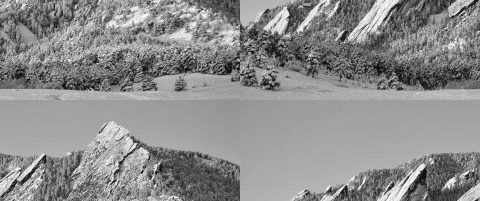
\includegraphics[scale=0.7]{./img/vhsg1.png}
    \caption{Photo 1 - Vertical and
    Horizontal Shift}
    \label{fig:p1vg}
  \end{subfigure}
  \begin{subfigure}{\textwidth}
    \centering
    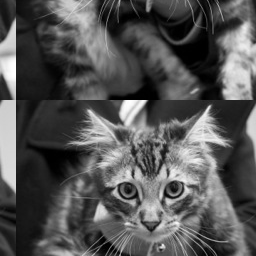
\includegraphics[scale=0.7]{./img/vhsg2.png}
    \caption{Photo
      2
      -
      Vertital
      and
      Horizontal
    Shift}
    \label{fig:p2vg}
  \end{subfigure}
  \caption{Vertically
    Shifted
  Images}
  \label{fig:vs_images}
\end{figure}

\section{Inversion}


\section{Transposition}

\section{Inversion}


\section{Restrictions on Compression with the Discrete Sine Transform}

With the given equation to transform images using the Discrete Sine Transform \eqref{eq:dst}, there does exist a limitation on the initial image aspect ratio -- the image \textit{must} by square. If it is not square, then the dot product will not work, and the image will not be compressed. The reason behind this is that since we are performing a dot product on the same matrix on either side, we know that in order for it to work it needs to be the same size after either operation is performed. The only matrix this holds true for is a square matrix.

That being said, the code below expresses a different algorithm. Instead of being limited to square matrices through the nuances of dot products, the code instead separates the two operations and performs them separately using two differently sized DST matrices. This algorithm is not limited by square matrices since it creates a new DST matrix for each operation.

    \lstinputlisting[language=Python,
                    showstringspaces=false,
                    frame=single,
                    firstline=181,
                    lastline=192,
                    basicstyle=\ttfamily,
                    keywordstyle=\color{blue},
                    numbers=left,
                    commentstyle=\color{red}]{./py/analysis.py}

\input{./tex/revdst.tex}
\section{Compression}

\section{Optimization}

Human vision has noticeable thresholds for the perception of light frequency. We are a lot more sensitive to lower frequencies compared to higher ones. JPEG image compression involves identifying high frequency pixel groupings and removing them from the image; less data in the image matrix means that it takes up less digital storage.  We can compress the image by using the DST to identify high frequency data. We can also vary the extent of compression using a variable “$p$,” which goes from 0 to 1 where 0 represents a blank image and 1 represents an uncompressed image. To see a demonstration of how different values of $p$ affect the image's quality, please either click \framebox{\href{http://will-farmer.com/diffeq/Project_2_matrices/img/comp1.gif}{this link}} or download it \attachfile{./img/comp1.gif}{here}.

Because our equation focusses only on the high frequency values of the image, we can eliminate many pixels before our brains register a degradation in quality. Below is a graph that shows how much data is removed from each image as $p$ gets larger.

    \begin{figure}[ht]
        \centering
        \begin{subfigure}{0.41\textwidth}
            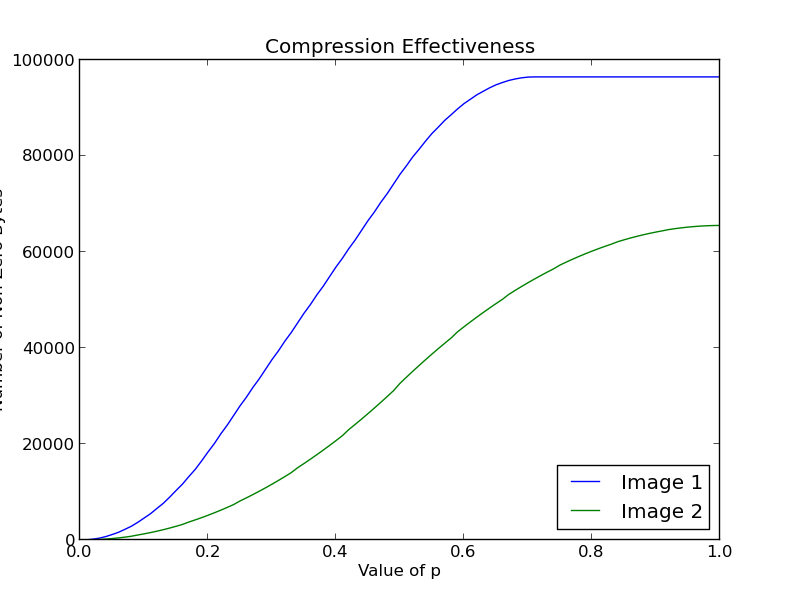
\includegraphics[scale=0.35]{./img/bitcount.png}
            \label{fig:bitcount}
            \caption{Bit Count vs. $p$ Value}
        \end{subfigure}
        \begin{subfigure}{0.41\textwidth}
            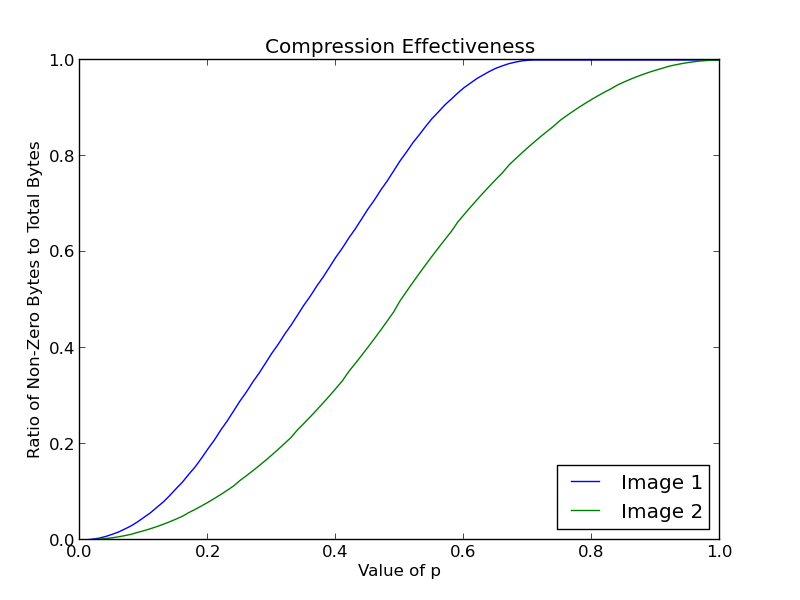
\includegraphics[scale=0.35]{./img/bitrat.png}
            \label{fig:bitrat}
            \caption{Bit Ratio vs. $p$ Value}
        \end{subfigure}
        \label{figs:bits}
    \end{figure}

Images can be compressed to low values of $p$ without being noticeable, especially if the images are primarily uniform and consist of low frequency pixels. This is because of the threshold frequencies in human vision.

Due to the inherent nature of images having different amounts of high frequency values, different values of $p$ will be appropriate for different images. For our first image, it initially will not have a large difference in quality as $p$ gets smaller, however for our last image it will immediately start reducing in size. Therefore different values of $P$ are appropriate for these different images.

\section{Conclusion}
Since digital images are represented as three dimensional matrices, image manipulation involves matrix operations. By using matrix multiplication, transpose, and the Discreet Sine Transformation (DST), we were able to translate, rotate, and compress multiple sized images. These analyses prove the usefulness of matrices when working with large sets of finite data, and they merely serve as an introduction to the powerful information processing that these tools provide.

To see all images produced from this project, please click \framebox{\href{http://will-farmer.com/diffeq/Project_2_matrices/img/}{this link}} and browse all of the images.

\section{Code}

The entire codebase for the project follows, and is available for download \attachfile{./code.tar.gz}{here}.\footnote{If you are unable to download these attached files, please go to \framebox{\href{http://will-farmer.com/diffeq/Project_2_matrices/code.tar.gz}{this link}}}

    \subsection{Python}

    The Python code to generate the images is included below.

        \lstinputlisting[language=Python,
                        showstringspaces=false,
                        frame=single,
                        basicstyle=\ttfamily,
                        keywordstyle=\color{blue},
                        numbers=left,
                        commentstyle=\color{red}]{./py/analysis.py}

    \newpage

    \subsection{MATLAB Code}

    Some MATLAB Code was also made that features equivalent functionality

        \subsubsection{Grayscale}

        \lstinputlisting[language=Matlab,
                        basicstyle=\ttfamily,
                        frame=single,
                        keywordstyle=\color{orange},
                        numbers=left,
                        commentstyle=\color{cyan}]{./mat/grayscale.m}

        \subsubsection{Horizontal Shifting}

        \lstinputlisting[language=Matlab,
                        basicstyle=\ttfamily,
                        frame=single,
                        keywordstyle=\color{orange},
                        numbers=left,
                        commentstyle=\color{cyan}]{./mat/hshift.m}

        \subsubsection{Vertical Shifting}

        \lstinputlisting[language=Matlab,
                        basicstyle=\ttfamily,
                        frame=single,
                        keywordstyle=\color{orange},
                        numbers=left,
                        commentstyle=\color{cyan}]{./mat/vshift.m}


\end{document}
